
\section*{Exercises}
\begin{enumerate}
    \item Evaluate $\biggl(\frac{\sqrt{e^x-1}}{x^2-x-6}\biggr)[x\leftrightarrows 4]$, being mindful to 
    indicate your serialization of the data.
    \item In the string \(f(x)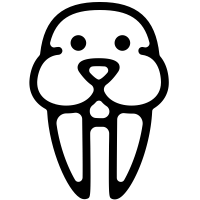
\includegraphics[width=0.5cm]{walrus.png} x\sqrt{x+2}\) 
    replace $x\leftrightarrows 4$ showing all the steps.  Is this $f(4)$? 
    What about in the string \(f(x)\defeq x\sqrt{x+2}\)?
\item Suppose $f(a/b)=a+b$.  Replace $a\leftrightarrows 1$ and $b\leftrightarrows 2$.  
Then do likewise with $a\leftrightarrows 2$ and $b\leftrightarrows 4$.  Does this show 
$f(1/2)\neq f(2/4)$?  

\end{enumerate}
